
\input{../../2021/style/preamble4tex}
% math spaces
\ifdefined\N                                                                
\renewcommand{\N}{\mathds{N}} % N, naturals
\else \newcommand{\N}{\mathds{N}} \fi 
\newcommand{\Z}{\mathds{Z}} % Z, integers
\newcommand{\Q}{\mathds{Q}} % Q, rationals
\newcommand{\R}{\mathds{R}} % R, reals
\ifdefined\C 
  \renewcommand{\C}{\mathds{C}} % C, complex
\else \newcommand{\C}{\mathds{C}} \fi
\newcommand{\continuous}{\mathcal{C}} % C, space of continuous functions
\newcommand{\M}{\mathcal{M}} % machine numbers
\newcommand{\epsm}{\epsilon_m} % maximum error

% counting / finite sets
\newcommand{\setzo}{\{0, 1\}} % set 0, 1
\newcommand{\setmp}{\{-1, +1\}} % set -1, 1
\newcommand{\unitint}{[0, 1]} % unit interval

% basic math stuff
\newcommand{\xt}{\tilde x} % x tilde
\newcommand{\argmax}{\operatorname{arg\,max}} % argmax
\newcommand{\argmin}{\operatorname{arg\,min}} % argmin
\newcommand{\argminlim}{\mathop{\mathrm{arg\,min}}\limits} % argmax with limits
\newcommand{\argmaxlim}{\mathop{\mathrm{arg\,max}}\limits} % argmin with limits  
\newcommand{\sign}{\operatorname{sign}} % sign, signum
\newcommand{\I}{\mathbb{I}} % I, indicator
\newcommand{\order}{\mathcal{O}} % O, order
\newcommand{\pd}[2]{\frac{\partial{#1}}{\partial #2}} % partial derivative
\newcommand{\floorlr}[1]{\left\lfloor #1 \right\rfloor} % floor
\newcommand{\ceillr}[1]{\left\lceil #1 \right\rceil} % ceiling

% sums and products
\newcommand{\sumin}{\sum\limits_{i=1}^n} % summation from i=1 to n
\newcommand{\sumim}{\sum\limits_{i=1}^m} % summation from i=1 to m
\newcommand{\sumjn}{\sum\limits_{j=1}^n} % summation from j=1 to p
\newcommand{\sumjp}{\sum\limits_{j=1}^p} % summation from j=1 to p
\newcommand{\sumik}{\sum\limits_{i=1}^k} % summation from i=1 to k
\newcommand{\sumkg}{\sum\limits_{k=1}^g} % summation from k=1 to g
\newcommand{\sumjg}{\sum\limits_{j=1}^g} % summation from j=1 to g
\newcommand{\meanin}{\frac{1}{n} \sum\limits_{i=1}^n} % mean from i=1 to n
\newcommand{\meanim}{\frac{1}{m} \sum\limits_{i=1}^m} % mean from i=1 to n
\newcommand{\meankg}{\frac{1}{g} \sum\limits_{k=1}^g} % mean from k=1 to g
\newcommand{\prodin}{\prod\limits_{i=1}^n} % product from i=1 to n
\newcommand{\prodkg}{\prod\limits_{k=1}^g} % product from k=1 to g
\newcommand{\prodjp}{\prod\limits_{j=1}^p} % product from j=1 to p

% linear algebra
\newcommand{\one}{\boldsymbol{1}} % 1, unitvector
\newcommand{\zero}{\mathbf{0}} % 0-vector
\newcommand{\id}{\boldsymbol{I}} % I, identity
\newcommand{\diag}{\operatorname{diag}} % diag, diagonal
\newcommand{\trace}{\operatorname{tr}} % tr, trace
\newcommand{\spn}{\operatorname{span}} % span
\newcommand{\scp}[2]{\left\langle #1, #2 \right\rangle} % <.,.>, scalarproduct
\newcommand{\mat}[1]{\begin{pmatrix} #1 \end{pmatrix}} % short pmatrix command
\newcommand{\Amat}{\mathbf{A}} % matrix A
\newcommand{\Deltab}{\mathbf{\Delta}} % error term for vectors

% basic probability + stats
\renewcommand{\P}{\mathds{P}} % P, probability
\newcommand{\E}{\mathds{E}} % E, expectation
\newcommand{\var}{\mathsf{Var}} % Var, variance
\newcommand{\cov}{\mathsf{Cov}} % Cov, covariance
\newcommand{\corr}{\mathsf{Corr}} % Corr, correlation
\newcommand{\normal}{\mathcal{N}} % N of the normal distribution
\newcommand{\iid}{\overset{i.i.d}{\sim}} % dist with i.i.d superscript
\newcommand{\distas}[1]{\overset{#1}{\sim}} % ... is distributed as ...

% machine learning
\newcommand{\Xspace}{\mathcal{X}} % X, input space
\newcommand{\Yspace}{\mathcal{Y}} % Y, output space
\newcommand{\nset}{\{1, \ldots, n\}} % set from 1 to n
\newcommand{\pset}{\{1, \ldots, p\}} % set from 1 to p
\newcommand{\gset}{\{1, \ldots, g\}} % set from 1 to g
\newcommand{\Pxy}{\mathbb{P}_{xy}} % P_xy
\newcommand{\Exy}{\mathbb{E}_{xy}} % E_xy: Expectation over random variables xy
\newcommand{\xv}{\mathbf{x}} % vector x (bold)
\newcommand{\xtil}{\tilde{\mathbf{x}}} % vector x-tilde (bold)
\newcommand{\yv}{\mathbf{y}} % vector y (bold)
\newcommand{\xy}{(\xv, y)} % observation (x, y)
\newcommand{\xvec}{\left(x_1, \ldots, x_p\right)^\top} % (x1, ..., xp) 
\newcommand{\Xmat}{\mathbf{X}} % Design matrix
\newcommand{\allDatasets}{\mathds{D}} % The set of all datasets
\newcommand{\allDatasetsn}{\mathds{D}_n}  % The set of all datasets of size n 
\newcommand{\D}{\mathcal{D}} % D, data
\newcommand{\Dn}{\D_n} % D_n, data of size n
\newcommand{\Dtrain}{\mathcal{D}_{\text{train}}} % D_train, training set
\newcommand{\Dtest}{\mathcal{D}_{\text{test}}} % D_test, test set
\newcommand{\xyi}[1][i]{\left(\xv^{(#1)}, y^{(#1)}\right)} % (x^i, y^i), i-th observation
\newcommand{\Dset}{\left( \xyi[1], \ldots, \xyi[n]\right)} % {(x1,y1)), ..., (xn,yn)}, data
\newcommand{\defAllDatasetsn}{(\Xspace \times \Yspace)^n} % Def. of the set of all datasets of size n 
\newcommand{\defAllDatasets}{\bigcup_{n \in \N}(\Xspace \times \Yspace)^n} % Def. of the set of all datasets 
\newcommand{\xdat}{\left\{ \xv^{(1)}, \ldots, \xv^{(n)}\right\}} % {x1, ..., xn}, input data
\newcommand{\yvec}{\left(y^{(1)}, \hdots, y^{(n)}\right)^\top} % (y1, ..., yn), vector of outcomes
\renewcommand{\xi}[1][i]{\xv^{(#1)}} % x^i, i-th observed value of x
\newcommand{\yi}[1][i]{y^{(#1)}} % y^i, i-th observed value of y 
\newcommand{\xivec}{\left(x^{(i)}_1, \ldots, x^{(i)}_p\right)^\top} % (x1^i, ..., xp^i), i-th observation vector
\newcommand{\xj}{\xv_j} % x_j, j-th feature
\newcommand{\xjvec}{\left(x^{(1)}_j, \ldots, x^{(n)}_j\right)^\top} % (x^1_j, ..., x^n_j), j-th feature vector
\newcommand{\phiv}{\mathbf{\phi}} % Basis transformation function phi
\newcommand{\phixi}{\mathbf{\phi}^{(i)}} % Basis transformation of xi: phi^i := phi(xi)

%%%%%% ml - models general
\newcommand{\lamv}{\bm{\lambda}} % lambda vector, hyperconfiguration vector
\newcommand{\Lam}{\bm{\Lambda}}	 % Lambda, space of all hpos
% Inducer / Inducing algorithm
\newcommand{\preimageInducer}{\left(\defAllDatasets\right)\times\Lam} % Set of all datasets times the hyperparameter space
\newcommand{\preimageInducerShort}{\allDatasets\times\Lam} % Set of all datasets times the hyperparameter space
% Inducer / Inducing algorithm
\newcommand{\ind}{\mathcal{I}} % Inducer, inducing algorithm, learning algorithm 

% continuous prediction function f
\newcommand{\ftrue}{f_{\text{true}}}  % True underlying function (if a statistical model is assumed)
\newcommand{\ftruex}{\ftrue(\xv)} % True underlying function (if a statistical model is assumed)
\newcommand{\fx}{f(\xv)} % f(x), continuous prediction function
\newcommand{\fdomains}{f: \Xspace \rightarrow \R^g} % f with domain and co-domain
\newcommand{\Hspace}{\mathcal{H}} % hypothesis space where f is from
\newcommand{\fbayes}{f^{\ast}} % Bayes-optimal model
\newcommand{\fxbayes}{f^{\ast}(\xv)} % Bayes-optimal model
\newcommand{\fkx}[1][k]{f_{#1}(\xv)} % f_j(x), discriminant component function
\newcommand{\fh}{\hat{f}} % f hat, estimated prediction function
\newcommand{\fxh}{\fh(\xv)} % fhat(x)
\newcommand{\fxt}{f(\xv ~|~ \thetab)} % f(x | theta)
\newcommand{\fxi}{f\left(\xv^{(i)}\right)} % f(x^(i))
\newcommand{\fxih}{\hat{f}\left(\xv^{(i)}\right)} % f(x^(i))
\newcommand{\fxit}{f\left(\xv^{(i)} ~|~ \thetab\right)} % f(x^(i) | theta)
\newcommand{\fhD}{\fh_{\D}} % fhat_D, estimate of f based on D
\newcommand{\fhDtrain}{\fh_{\Dtrain}} % fhat_Dtrain, estimate of f based on D
\newcommand{\fhDnlam}{\fh_{\Dn, \lamv}} %model learned on Dn with hp lambda
\newcommand{\fhDlam}{\fh_{\D, \lamv}} %model learned on D with hp lambda
\newcommand{\fhDnlams}{\fh_{\Dn, \lamv^\ast}} %model learned on Dn with optimal hp lambda 
\newcommand{\fhDlams}{\fh_{\D, \lamv^\ast}} %model learned on D with optimal hp lambda 

% discrete prediction function h
\newcommand{\hx}{h(\xv)} % h(x), discrete prediction function
\newcommand{\hh}{\hat{h}} % h hat
\newcommand{\hxh}{\hat{h}(\xv)} % hhat(x)
\newcommand{\hxt}{h(\xv | \thetab)} % h(x | theta)
\newcommand{\hxi}{h\left(\xi\right)} % h(x^(i))
\newcommand{\hxit}{h\left(\xi ~|~ \thetab\right)} % h(x^(i) | theta)
\newcommand{\hbayes}{h^{\ast}} % Bayes-optimal classification model
\newcommand{\hxbayes}{h^{\ast}(\xv)} % Bayes-optimal classification model

% yhat
\newcommand{\yh}{\hat{y}} % yhat for prediction of target
\newcommand{\yih}{\hat{y}^{(i)}} % yhat^(i) for prediction of ith targiet
\newcommand{\resi}{\yi- \yih}

% theta
\newcommand{\thetah}{\hat{\theta}} % theta hat
\newcommand{\thetab}{\bm{\theta}} % theta vector
\newcommand{\thetabh}{\bm{\hat\theta}} % theta vector hat
\newcommand{\thetat}[1][t]{\thetab^{[#1]}} % theta^[t] in optimization
\newcommand{\thetatn}[1][t]{\thetab^{[#1 +1]}} % theta^[t+1] in optimization
\newcommand{\thetahDnlam}{\thetabh_{\Dn, \lamv}} %theta learned on Dn with hp lambda
\newcommand{\thetahDlam}{\thetabh_{\D, \lamv}} %theta learned on D with hp lambda
\newcommand{\mint}{\min_{\thetab \in \Theta}} % min problem theta
\newcommand{\argmint}{\argmin_{\thetab \in \Theta}} % argmin theta

% densities + probabilities
% pdf of x 
\newcommand{\pdf}{p} % p
\newcommand{\pdfx}{p(\xv)} % p(x)
\newcommand{\pixt}{\pi(\xv~|~ \thetab)} % pi(x|theta), pdf of x given theta
\newcommand{\pixit}{\pi\left(\xi ~|~ \thetab\right)} % pi(x^i|theta), pdf of x given theta
\newcommand{\pixii}{\pi\left(\xi\right)} % pi(x^i), pdf of i-th x 

% pdf of (x, y)
\newcommand{\pdfxy}{p(\xv,y)} % p(x, y)
\newcommand{\pdfxyt}{p(\xv, y ~|~ \thetab)} % p(x, y | theta)
\newcommand{\pdfxyit}{p\left(\xi, \yi ~|~ \thetab\right)} % p(x^(i), y^(i) | theta)

% pdf of x given y
\newcommand{\pdfxyk}[1][k]{p(\xv | y= #1)} % p(x | y = k)
\newcommand{\lpdfxyk}[1][k]{\log p(\xv | y= #1)} % log p(x | y = k)
\newcommand{\pdfxiyk}[1][k]{p\left(\xi | y= #1 \right)} % p(x^i | y = k)

% prior probabilities
\newcommand{\pik}[1][k]{\pi_{#1}} % pi_k, prior
\newcommand{\lpik}[1][k]{\log \pi_{#1}} % log pi_k, log of the prior
\newcommand{\pit}{\pi(\thetab)} % Prior probability of parameter theta

% posterior probabilities
\newcommand{\post}{\P(y = 1 ~|~ \xv)} % P(y = 1 | x), post. prob for y=1
\newcommand{\postk}[1][k]{\P(y = #1 ~|~ \xv)} % P(y = k | y), post. prob for y=k
\newcommand{\pidomains}{\pi: \Xspace \rightarrow \unitint} % pi with domain and co-domain
\newcommand{\pibayes}{\pi^{\ast}} % Bayes-optimal classification model
\newcommand{\pixbayes}{\pi^{\ast}(\xv)} % Bayes-optimal classification model
\newcommand{\pix}{\pi(\xv)} % pi(x), P(y = 1 | x)
\newcommand{\pikx}[1][k]{\pi_{#1}(\xv)} % pi_k(x), P(y = k | x)
\newcommand{\pikxt}[1][k]{\pi_{#1}(\xv ~|~ \thetab)} % pi_k(x | theta), P(y = k | x, theta)
\newcommand{\pixh}{\hat \pi(\xv)} % pi(x) hat, P(y = 1 | x) hat
\newcommand{\pikxh}[1][k]{\hat \pi_{#1}(\xv)} % pi_k(x) hat, P(y = k | x) hat
\newcommand{\pixih}{\hat \pi(\xi)} % pi(x^(i)) with hat
\newcommand{\pikxih}[1][k]{\hat \pi_{#1}(\xi)} % pi_k(x^(i)) with hat
\newcommand{\pdfygxt}{p(y ~|~\xv, \thetab)} % p(y | x, theta)
\newcommand{\pdfyigxit}{p\left(\yi ~|~\xi, \thetab\right)} % p(y^i |x^i, theta)
\newcommand{\lpdfygxt}{\log \pdfygxt } % log p(y | x, theta)
\newcommand{\lpdfyigxit}{\log \pdfyigxit} % log p(y^i |x^i, theta)

% probababilistic
\newcommand{\bayesrulek}[1][k]{\frac{\P(\xv | y= #1) \P(y= #1)}{\P(\xv)}} % Bayes rule
\newcommand{\muk}{\bm{\mu_k}} % mean vector of class-k Gaussian (discr analysis) 

% residual and margin
\newcommand{\eps}{\epsilon} % residual, stochastic
\newcommand{\epsi}{\epsilon^{(i)}} % epsilon^i, residual, stochastic
\newcommand{\epsh}{\hat{\epsilon}} % residual, estimated
\newcommand{\yf}{y \fx} % y f(x), margin
\newcommand{\yfi}{\yi \fxi} % y^i f(x^i), margin
\newcommand{\Sigmah}{\hat \Sigma} % estimated covariance matrix
\newcommand{\Sigmahj}{\hat \Sigma_j} % estimated covariance matrix for the j-th class

% ml - loss, risk, likelihood
\newcommand{\Lyf}{L\left(y, f\right)} % L(y, f), loss function
\newcommand{\Lxy}{L\left(y, \fx\right)} % L(y, f(x)), loss function
\newcommand{\Lxyi}{L\left(\yi, \fxi\right)} % loss of observation
\newcommand{\Lxyt}{L\left(y, \fxt\right)} % loss with f parameterized
\newcommand{\Lxyit}{L\left(\yi, \fxit\right)} % loss of observation with f parameterized
\newcommand{\Lxym}{L\left(\yi, f\left(\bm{\tilde{x}}^{(i)} ~|~ \thetab\right)\right)} % loss of observation with f parameterized
\newcommand{\Lpixy}{L\left(y, \pix\right)} % loss in classification
\newcommand{\Lpixyi}{L\left(\yi, \pixii\right)} % loss of observation in classification
\newcommand{\Lpixyt}{L\left(y, \pixt\right)} % loss with pi parameterized
\newcommand{\Lpixyit}{L\left(\yi, \pixit\right)} % loss of observation with pi parameterized
\newcommand{\Lhxy}{L\left(y, \hx\right)} % L(y, h(x)), loss function on discrete classes
\newcommand{\Lr}{L\left(r\right)} % L(r), loss defined on residual (reg) / margin (classif)
\newcommand{\lone}{|y - \fx|} % L1 loss
\newcommand{\ltwo}{\left(y - \fx\right)^2} % L2 loss
\newcommand{\lbernoullimp}{\ln(1 + \exp(-y \cdot \fx))} % Bernoulli loss for -1, +1 encoding
\newcommand{\lbernoullizo}{- y \cdot \fx + \log(1 + \exp(\fx))} % Bernoulli loss for 0, 1 encoding
\newcommand{\lcrossent}{- y \log \left(\pix\right) - (1 - y) \log \left(1 - \pix\right)} % cross-entropy loss
\newcommand{\lbrier}{\left(\pix - y \right)^2} % Brier score
\newcommand{\risk}{\mathcal{R}} % R, risk
\newcommand{\riskbayes}{\mathcal{R}^\ast}
\newcommand{\riskf}{\risk(f)} % R(f), risk
\newcommand{\riskdef}{\E_{y|\xv}\left(\Lxy \right)} % risk def (expected loss)
\newcommand{\riskt}{\mathcal{R}(\thetab)} % R(theta), risk
\newcommand{\riske}{\mathcal{R}_{\text{emp}}} % R_emp, empirical risk w/o factor 1 / n
\newcommand{\riskeb}{\bar{\mathcal{R}}_{\text{emp}}} % R_emp, empirical risk w/ factor 1 / n
\newcommand{\riskef}{\riske(f)} % R_emp(f)
\newcommand{\risket}{\mathcal{R}_{\text{emp}}(\thetab)} % R_emp(theta)
\newcommand{\riskr}{\mathcal{R}_{\text{reg}}} % R_reg, regularized risk
\newcommand{\riskrt}{\mathcal{R}_{\text{reg}}(\thetab)} % R_reg(theta)
\newcommand{\riskrf}{\riskr(f)} % R_reg(f)
\newcommand{\riskrth}{\hat{\mathcal{R}}_{\text{reg}}(\thetab)} % hat R_reg(theta)
\newcommand{\risketh}{\hat{\mathcal{R}}_{\text{emp}}(\thetab)} % hat R_emp(theta)
\newcommand{\LL}{\mathcal{L}} % L, likelihood
\newcommand{\LLt}{\mathcal{L}(\thetab)} % L(theta), likelihood
\newcommand{\LLtx}{\mathcal{L}(\thetab | \xv)} % L(theta|x), likelihood
\newcommand{\logl}{\ell} % l, log-likelihood
\newcommand{\loglt}{\logl(\thetab)} % l(theta), log-likelihood
\newcommand{\logltx}{\logl(\thetab | \xv)} % l(theta|x), log-likelihood
\newcommand{\errtrain}{\text{err}_{\text{train}}} % training error
\newcommand{\errtest}{\text{err}_{\text{test}}} % test error
\newcommand{\errexp}{\overline{\text{err}_{\text{test}}}} % avg training error

% lm
\newcommand{\thx}{\thetab^\top \xv} % linear model
\newcommand{\olsest}{(\Xmat^\top \Xmat)^{-1} \Xmat^\top \yv} % OLS estimator in LM 

\input{../../latex-math/ml-bagging.tex}
\input{../../latex-math/ml-boosting.tex}
% ml - trees, extra trees

\newcommand{\Np}{\mathcal{N}} % (Parent) node N
\newcommand{\Npk}{\Np_k} % node N_k
\newcommand{\Nl}{\Np_1}	% Left node N_1
\newcommand{\Nr}{\Np_2} % Right node N_2
\newcommand{\pikN}[1][k]{\pi_#1^{(\Np)}} % class probability node N
\newcommand{\pikNh}[1][k]{\hat\pi_#1^{(\Np)}} % estimated class probability node N
\newcommand{\pikNlh}[1][k]{\hat\pi_#1^{(\Nl)}} % estimated class probability left node
\newcommand{\pikNrh}[1][k]{\hat\pi_#1^{(\Nr)}} % estimated class probability right node


\begin{document}

\lecturechapter{11}{Gradient Boosting with Trees}
\lecture{Fortgeschrittene Computerintensive Methoden}


\begin{vbframe}{Gradient boosting with trees}

Trees are mainly used as base learners for gradient boosting in ML.
A great deal of research has been done on this combination so far, and it often provides the best results.

\begin{blocki}{Reminder: Advantages of trees}
\item No problems with categorical features.
\item No problems with outliers in feature values.
\item No problems with missing values.
\item No problems with monotone transformations of features.
\item Trees (and stumps!) can be fitted quickly, even for large $n$.
\item Trees have a simple built-in type of variable selection.
%\item Interpretation of Trees is rather easy.
\end{blocki}
The gradient-boosted trees method retains all of them, and strongly improves the trees' predictive power.
Furthermore, it is possible to adapt gradient boosting to tree learners in a targeted manner.

\framebreak

One can write a tree as: $ b(\xv) = \sum_{t=1}^{T} c_t \mathds{1}_{\{\xv \in R_t\}} $,
where $R_t$ are the terminal regions and $c_t$ the corresponding constant parameter.

\vspace*{0.2cm}

For a fitted tree with regions $R_t$, the special additive structure can be exploited in boosting:  %Finished here

\begin{align*}
  \fm(\xv) &= \fmd(\xv) +  \betam \bmm(\xv) \\
         &= \fmd(\xv) +  \betam \sum_{t=1}^{\Tm} \ctm \mathds{1}_{\{\xv \in \Rtm\}}.
\end{align*}

Actually, we do not have to find $\ctm$ and $\betam$ in two separate steps
(fitting against pseudo-residuals, then line search) but find optimal $\ctm$ (including $\betam$).
Also note that the $\ctm$ will not really be loss-optimal as we used squared error loss
to fit them against the pseudo-residuals.

\framebreak
\begin{footnotesize}
We do the same steps as before: (1) calculate the pseudo-residuals, (2) fit a tree against pseudo-residuals, \textbf{but now} we keep only the structure of the tree and optimize the $c$ parameter in a (further) post-hoc step.

$$
\fm(\xv) = \fmd(\xv) +  \sum_{t=1}^{\Tm} \ctmt \mathds{1}_{\{\xv \in \Rtm\}}. 
$$

We want to find the constant value $c$ that drives down risk the most w.r.t the squared error loss,
when added to the respective terminal region.
We can determine/change all $\ctmt$ individually and directly $L$-optimally:


%\vspace{-0.2cm}

$$ \ctmt = \argmin_{c} \sum_{\xi \in \Rtm} L(\yi, \fmd(\xi) + c). $$

\vspace{-0.5cm}

\begin{center}

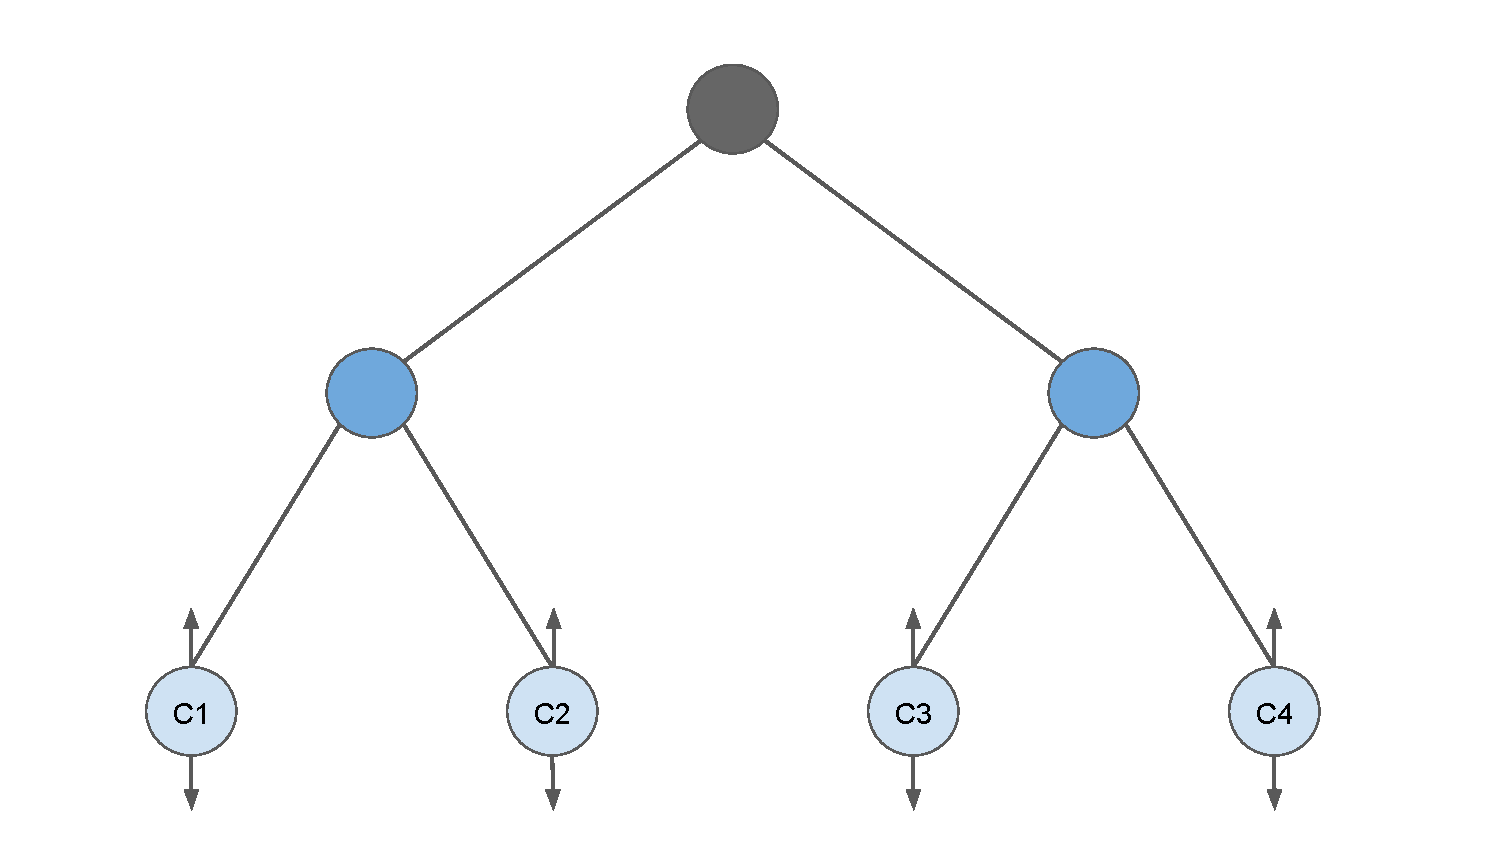
\includegraphics[width=0.38\textwidth]{figure_man/gbm_leaf_adjustment.pdf}

\end{center}

\end{footnotesize}

\framebreak

\begin{algorithm}[H]
  \begin{footnotesize}
  \begin{center}
  \caption{Gradient Tree Boosting Algorithm.}
    \begin{algorithmic}[1]
      \State Initialize $\hat{f}^{[0]}(\xv) = \argmin_{\theta} \sumin L(\yi, \theta)$
      \For{$m = 1 \to M$}
          \State For all $i$: $\rmi = -\left[\pd{\Lxyi}{\fxi}\right]_{f=\fmdh}$
          \State Fit regr. tree to the $\rmi$, giving terminal regions $\Rtm,
          \ t = 1,\ldots,\Tm$
        \For{$t = 1 \to \Tm$}
          \State $\ctmh = \argmin_{c} \sum \limits_{\xi \in \Rtm} L(\yi, \fmdh(\xi) + c)$
        \EndFor
        \State $\bmmh(\xv) = \sum_{t=1}^{T} \ctmh \mathds{1}_{\{x \in R_t\}} $
        \State Update $\fmh(\xv) = \fmdh(\xv) + \bmmh(\xv)$
      \EndFor
      \State Output $\hat{f}(\xv) = \hat{f}^{[M]}(\xv)$
    \end{algorithmic}
    \end{center}
    \end{footnotesize}
\end{algorithm}


\end{vbframe}


\begin{vbframe}{Visualization 1}
\begin{footnotesize}
\textbf{Simulation Setting:}
\begin{itemize}
\item Given: One feature $\xv$ and one numeric target variable $y$ of 50 observations.
\item $\xv$ is uniformly distributed between 0 and 10.
\item $y$ depends on $\xv$ as follows: $y^{(i)} = \sin{(x^{(i)})} + \epsilon^{(i)}$ with $\epsilon^{(i)} \sim \mathcal{N}(0,0.2)$, $\forall i \in 1,\dots,50$.
\end{itemize}

\vspace*{0.2cm}

\begin{columns}

\column{5cm}
\begin{figure}
  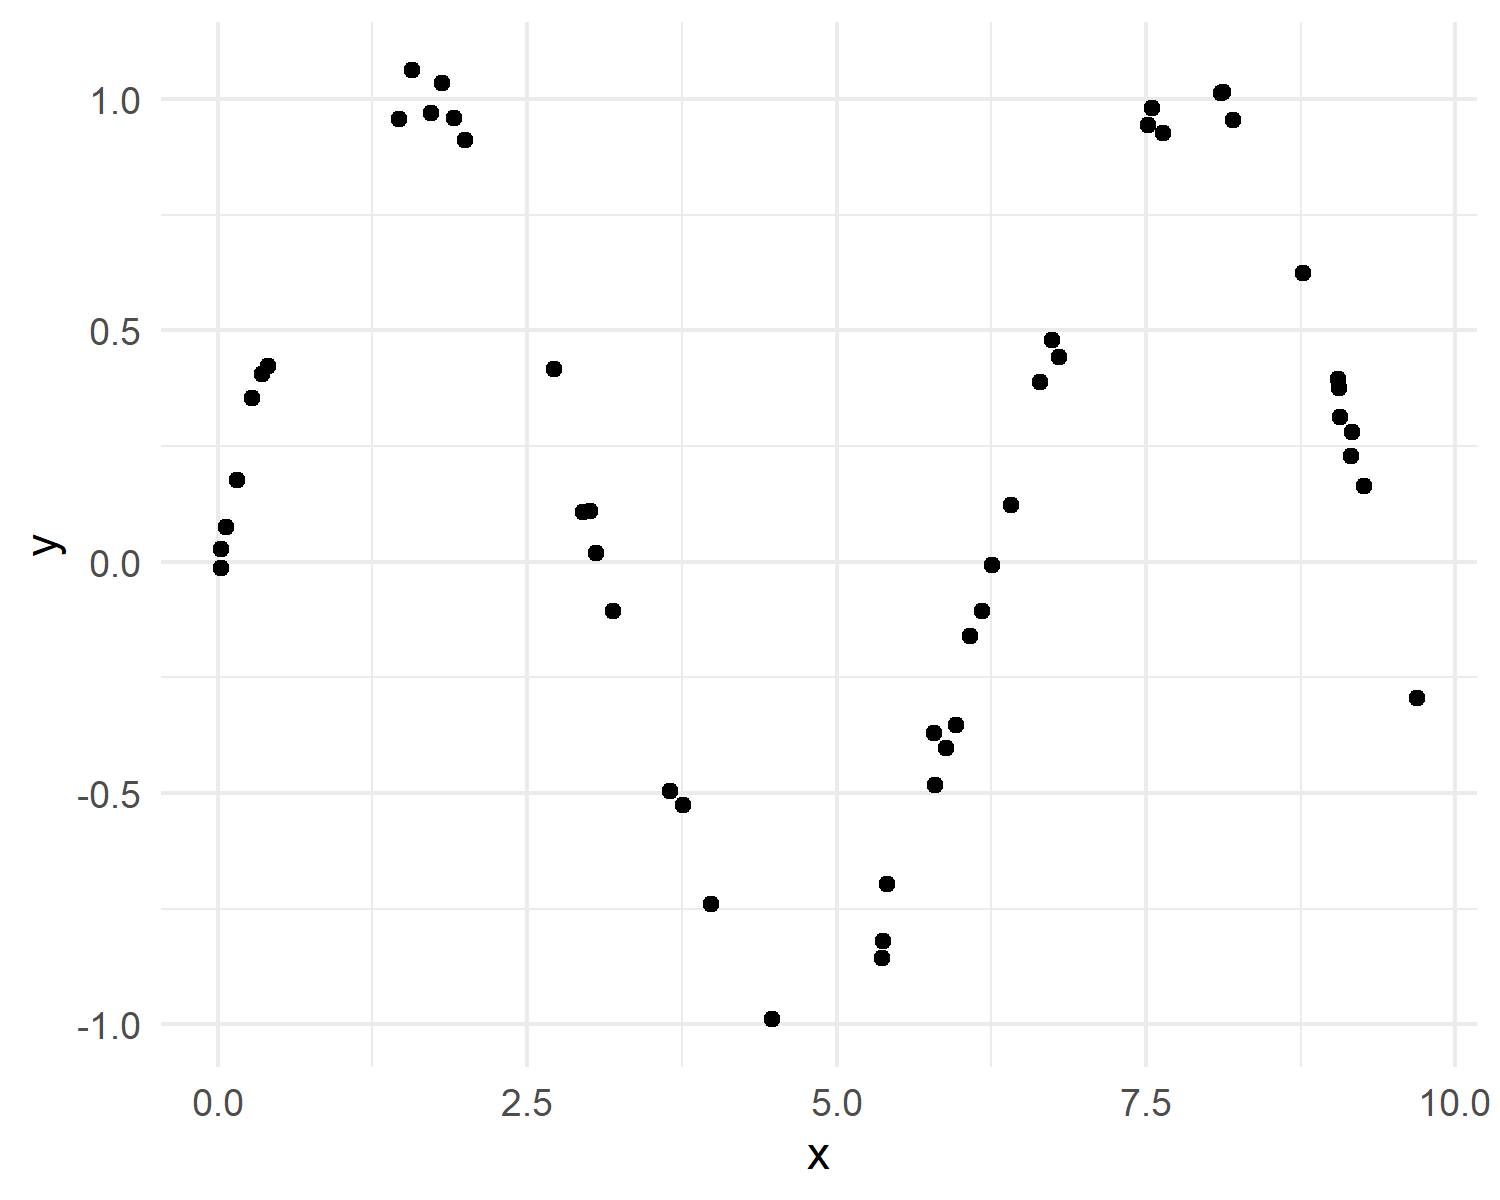
\includegraphics{figure_man/gbm_anim_data.png}
\end{figure}

\column{5cm}
\textbf{Aim:} We want to fit a gradient boosting model to the data by using stumps as base learners.
\begin{itemize}
\item Since we are facing a regression problem, we use L2 loss.
%\item Self-implementation of GB where learning rate found by line search.
\end{itemize}


\end{columns}
\end{footnotesize}
\framebreak

\begin{footnotesize}
\textbf{Iteration 0:} Initialization by optimal constant (mean) prediction $\hat f^{[0](i)}(\xv) = \overline{y} \approx 0.2$

\vspace*{0.2cm}

\begin{columns}

\column{5cm}
\begin{center}
\begin{tabular}{c|c|c|c}
$i$ & $x^{(i)}$ & $y^{(i)}$ & $\hat{f}^{[0]}$ \\ \hline
1 & 0.03 &  0.03 & 0.20 \\
2 & 0.03 & -0.01 & 0.20 \\
3 & 0.06 &  0.08 & 0.20 \\
\vdots & \vdots & \vdots & \vdots \\
50 & 9.69 & -0.29 & 0.20\\
\end{tabular}
\end{center}

\column{5cm}
\begin{figure}
  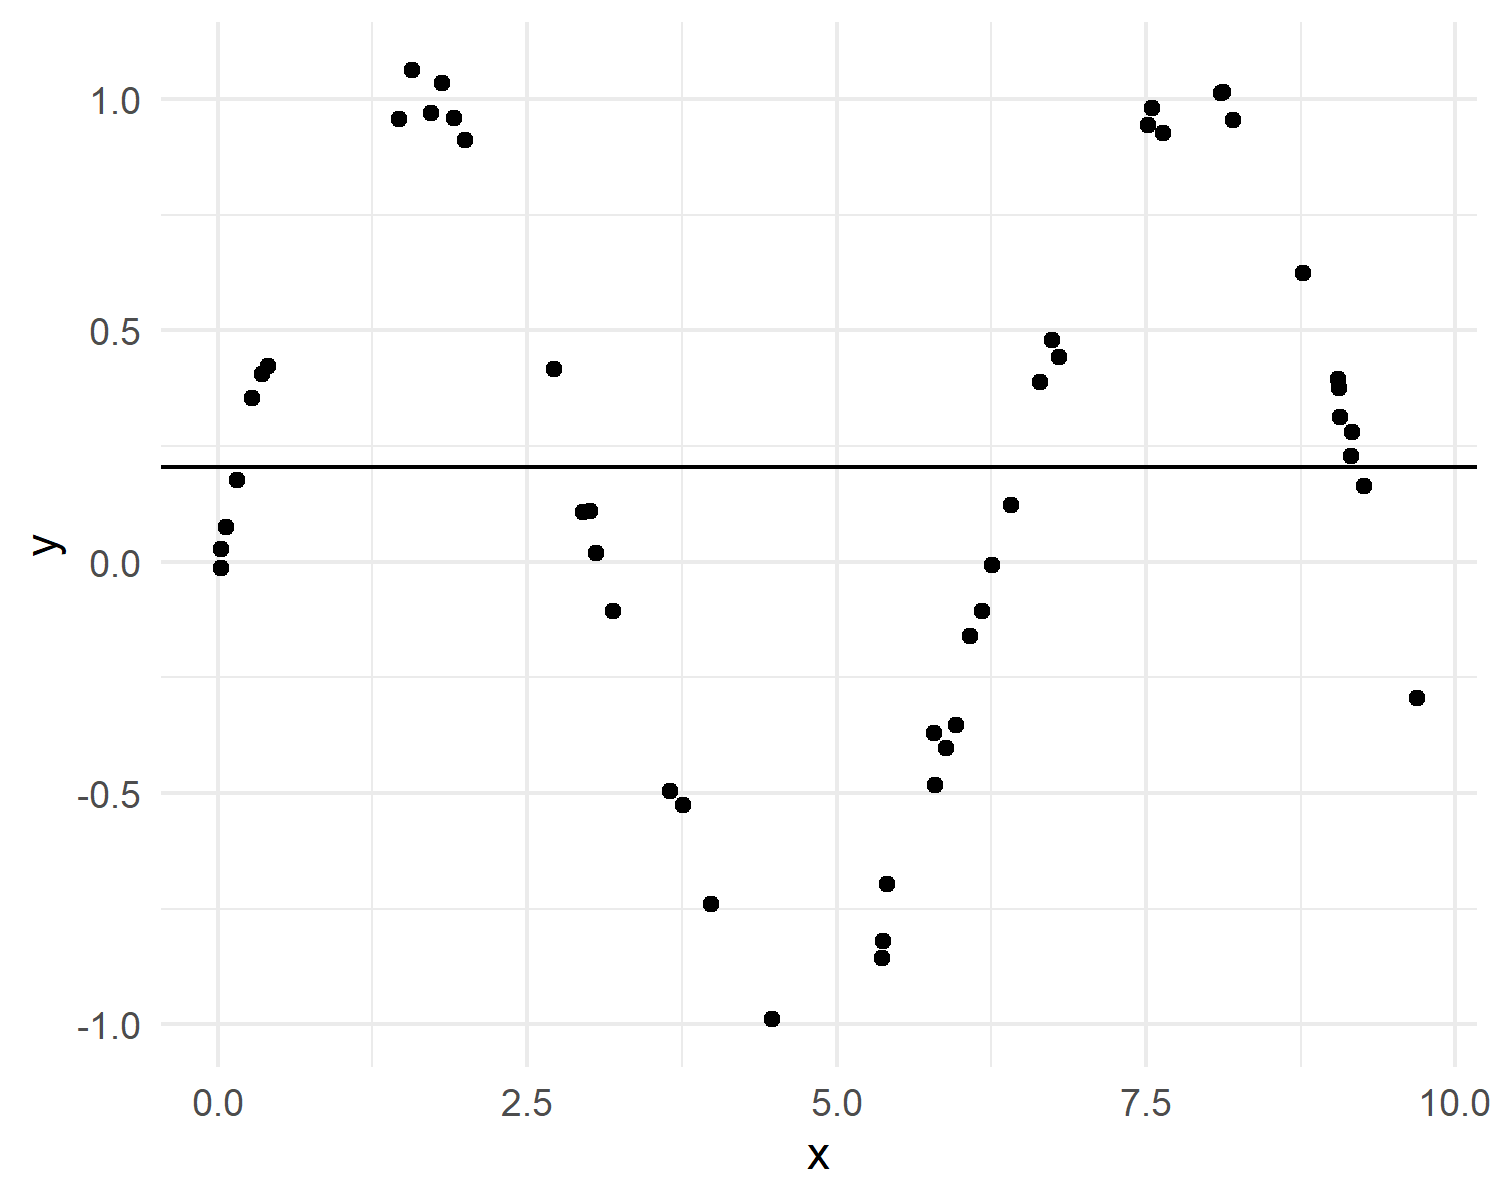
\includegraphics[width=\textwidth]{figure_man/gbm_anim_init.png}
\end{figure}

\end{columns}

\end{footnotesize}

\framebreak
\begin{footnotesize}
\textbf{Iteration 1:} (1) Calculate residuals $\tilde{r}^{[m](i)}$ and (2) fit a regression stump $b^{[m]}$ %which is multiplied by the learning rate $\beta$% (here: $\hat \beta^{[1]} = 1$).

\begin{columns}

\column{5cm}
\begin{center}
\begin{tabular}{c|c|c|c|c|c}
$i$ & $x^{(i)}$ & $y^{(i)}$ & $\hat{f}^{[0]}$ & $\tilde{r}^{[1](i)}$ & $\hat{b}^{[1](i)}$\\ \hline
1 & 0.03 &  0.03 & 0.20 & -0.17 & -0.18\\
2 & 0.03 & -0.01 & 0.20 & -0.21 & -0.18 \\
3 & 0.06 &  0.08 & 0.20 & -0.12 & -0.18 \\
\vdots & \vdots & \vdots & \vdots  & \vdots & \vdots \\
50 & 9.69 & -0.29 & 0.20 & -0.49 & 0.34\\
\end{tabular}
\end{center}

\column{4.9cm}
\begin{figure}
  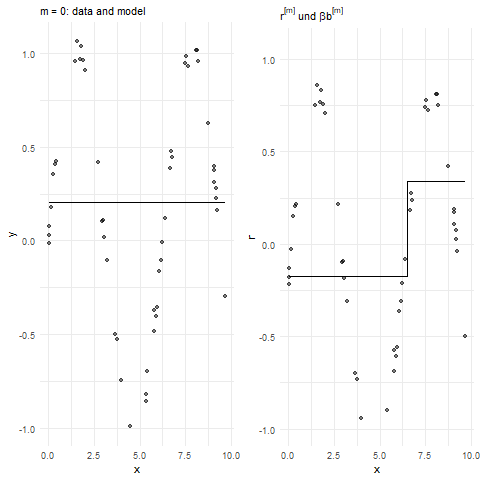
\includegraphics[width=\textwidth]{figure_man/gbm_anim_01.png}
\end{figure}

\end{columns}

\vspace*{0.2cm}

%(3) Update model by $\hat{f}^{[1]}(\xv) = \hat{f}^{[0]}(\xv) + \hat{\beta}^{[1]} \hat{b}^{[1]$
(3) Update model by $\hat{f}^{[1]}(\xv) = \hat{f}^{[0]}(\xv) + \hat{b}^{[1]$
\end{footnotesize}


\end{vbframe}

\begin{frame}{Visualization 1}
Repeat step (1) to (3):
\begin{center}
\only<1>{ 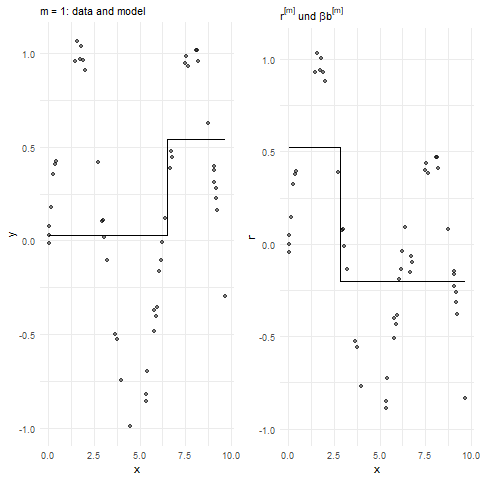
\includegraphics[width=0.6\textwidth]{figure_man/gbm_anim_02.png} }
\only<2>{ 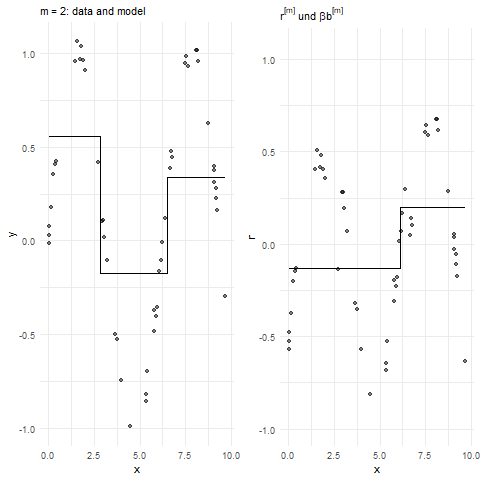
\includegraphics[width=0.6\textwidth]{figure_man/gbm_anim_03.png} }
\only<3>{ 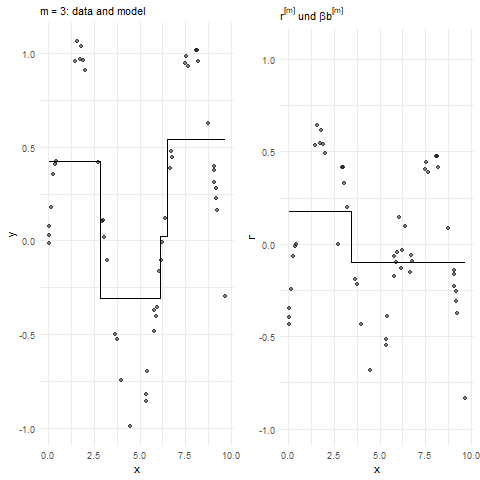
\includegraphics[width=0.6\textwidth]{figure_man/gbm_anim_04.png} }
\only<4>{ 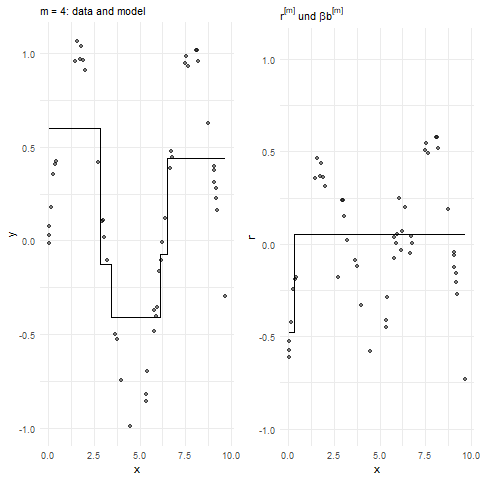
\includegraphics[width=0.6\textwidth]{figure_man/gbm_anim_05.png} }
\only<5>{ 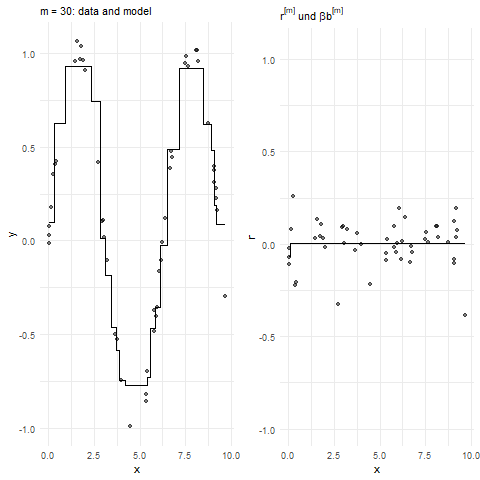
\includegraphics[width=0.6\textwidth]{figure_man/gbm_anim_31.png} }
\end{center}

\end{frame}
% 
% \begin{columns}
% \begin{column}{0.6\textwidth}
% \begin{center}
% \only<1>{ 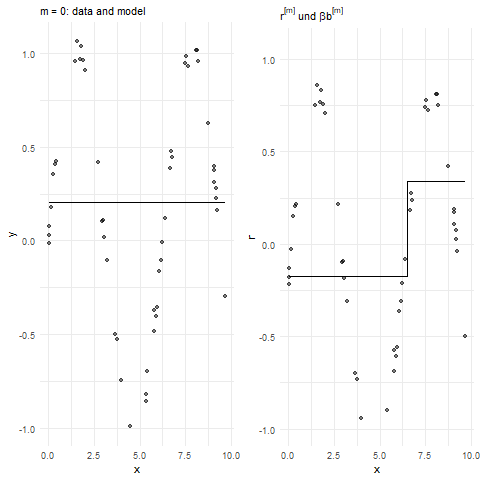
\includegraphics[width=\textwidth]{figure_man/gbm_anim_01.png} }
% \only<2>{ 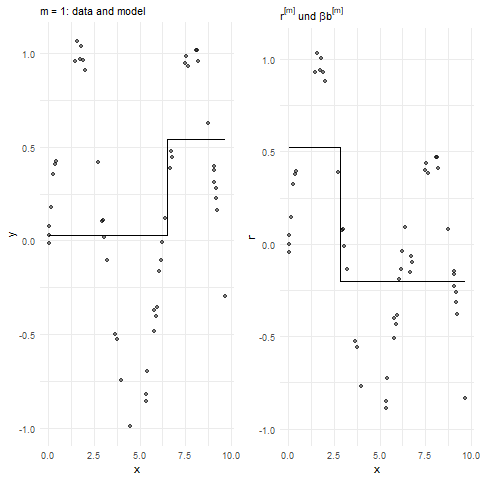
\includegraphics[width=\textwidth]{figure_man/gbm_anim_02.png} }
% \only<3>{ 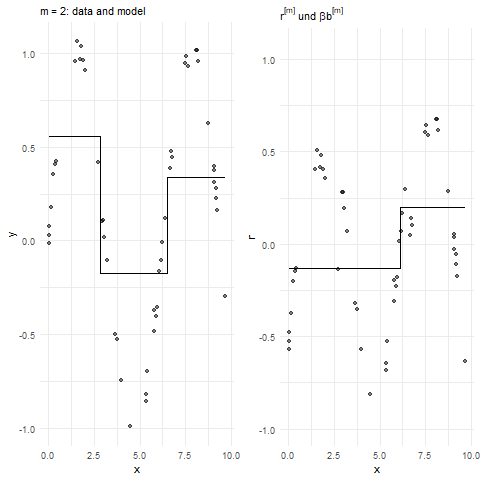
\includegraphics[width=\textwidth]{figure_man/gbm_anim_03.png} }
% \only<4>{ 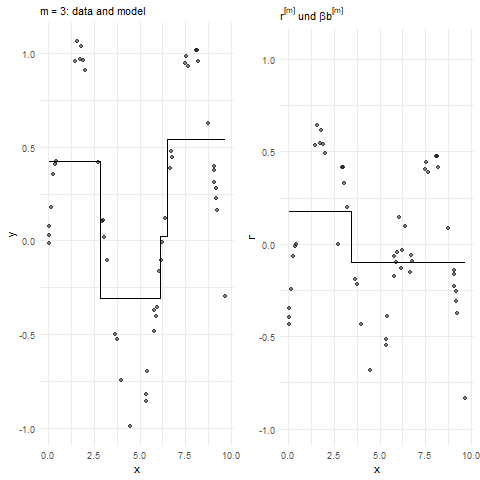
\includegraphics[width=\textwidth]{figure_man/gbm_anim_04.png} }
% \only<5>{ 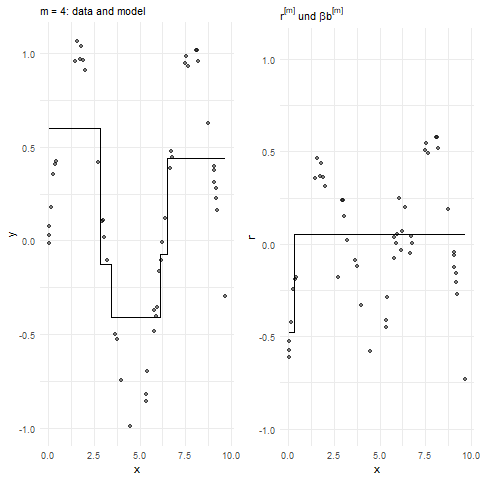
\includegraphics[width=\textwidth]{figure_man/gbm_anim_05.png} }
% \only<6>{ 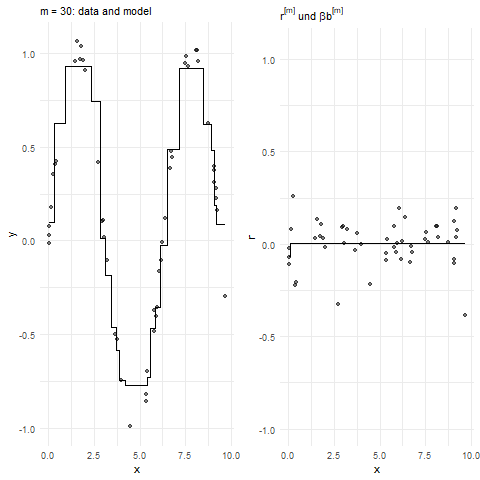
\includegraphics[width=\textwidth]{figure_man/gbm_anim_31.png} }
% \end{center}
% \end{column}
% \begin{column}{0.4\textwidth}
% \begin{itemize}
% \item L2 loss and stumps.
% \item Left = current additive model.
% \item Right = Residuals and fitted base learner.
% \item Plot is created by a self-implementation of GB where step size found by line search.
% \end{itemize}
% \end{column}
% \end{columns}
% \end{frame}

\begin{vbframe}{Visualization 2}

\vspace{-0.6cm}
\begin{center}
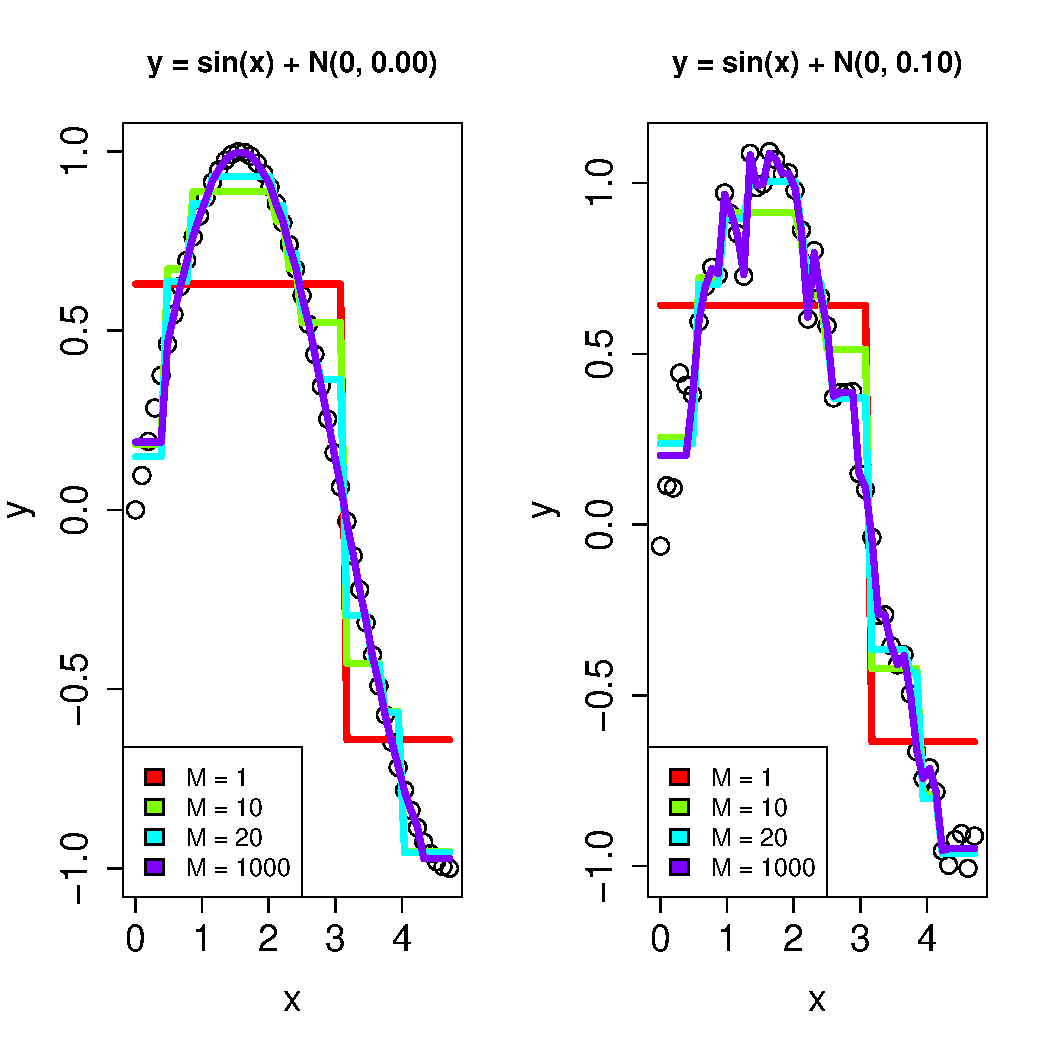
\includegraphics[width=0.6\textwidth]{figure_man/gbm_sine.pdf}
\end{center}

\vspace{-0.8cm}
\footnotesize
\begin{itemize}

  \item
    Iterating this very simple base learner yields a rather nice approximation of a smooth model in the end.

  \item
    Severe overfitting apparent in the noisy case. We will discuss and solve this problem later.

\end{itemize}

\end{vbframe}

\begin{vbframe}{Visualization 3}
\begin{center}
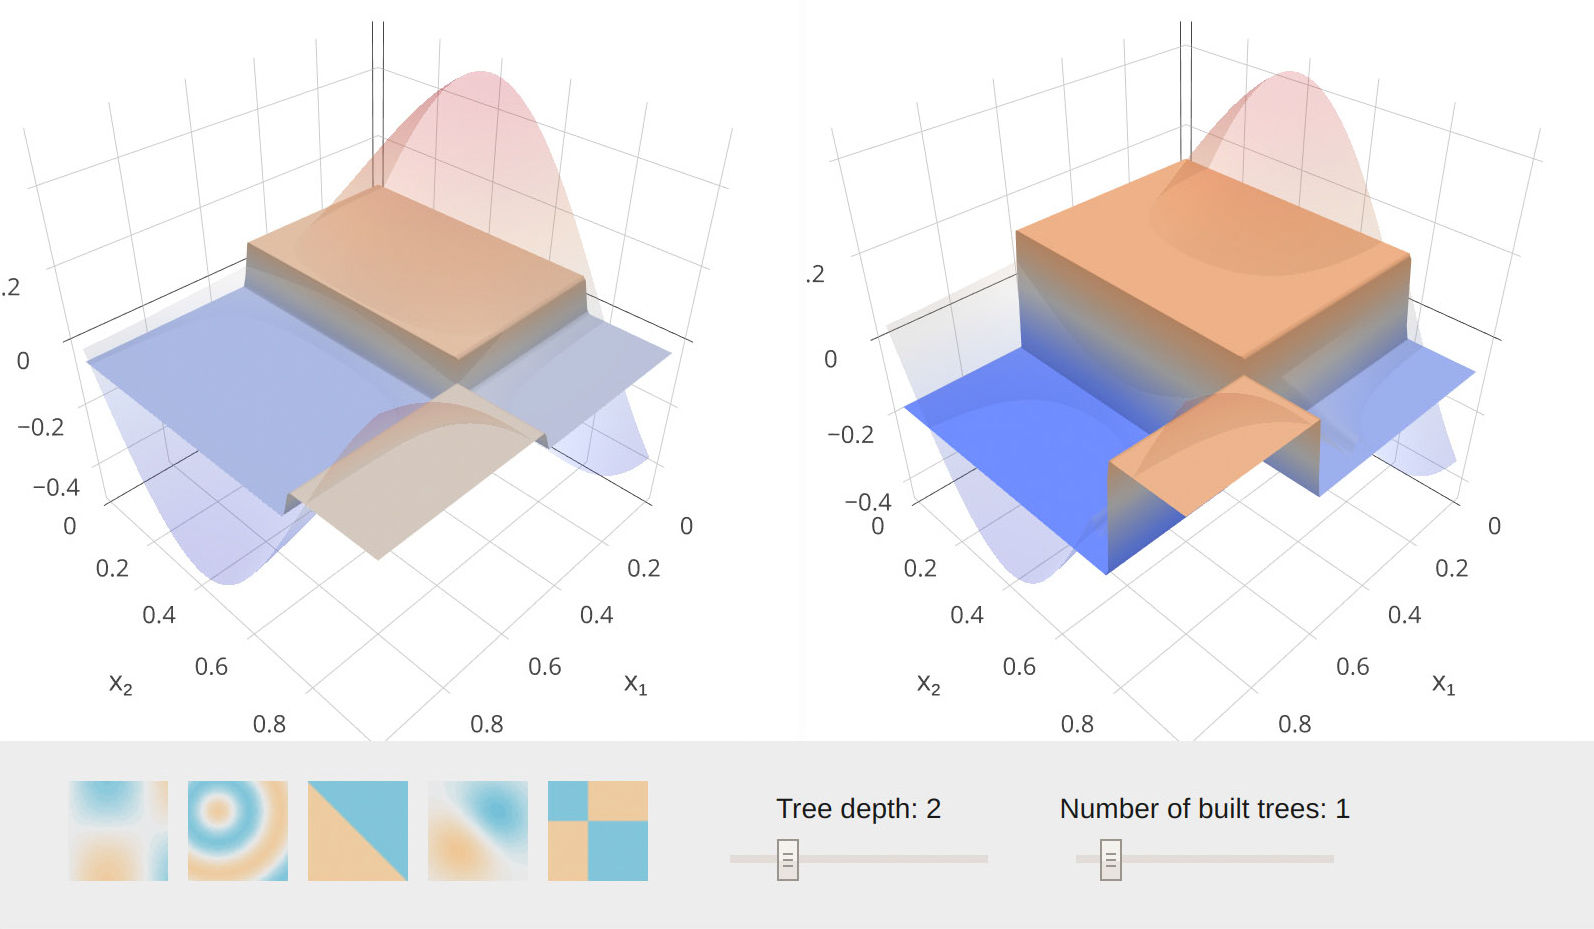
\includegraphics[width=\textwidth]{figure_man/gbm_anim/gbm1.jpg}
\href{http://arogozhnikov.github.io/2016/06/24/gradient_boosting_explained.html}{\beamergotobutton{Open in browser.}}
\end{center}
\end{vbframe}

% \begin{vbframe}{Gradient Boosting Visualization}
% \begin{center}
% 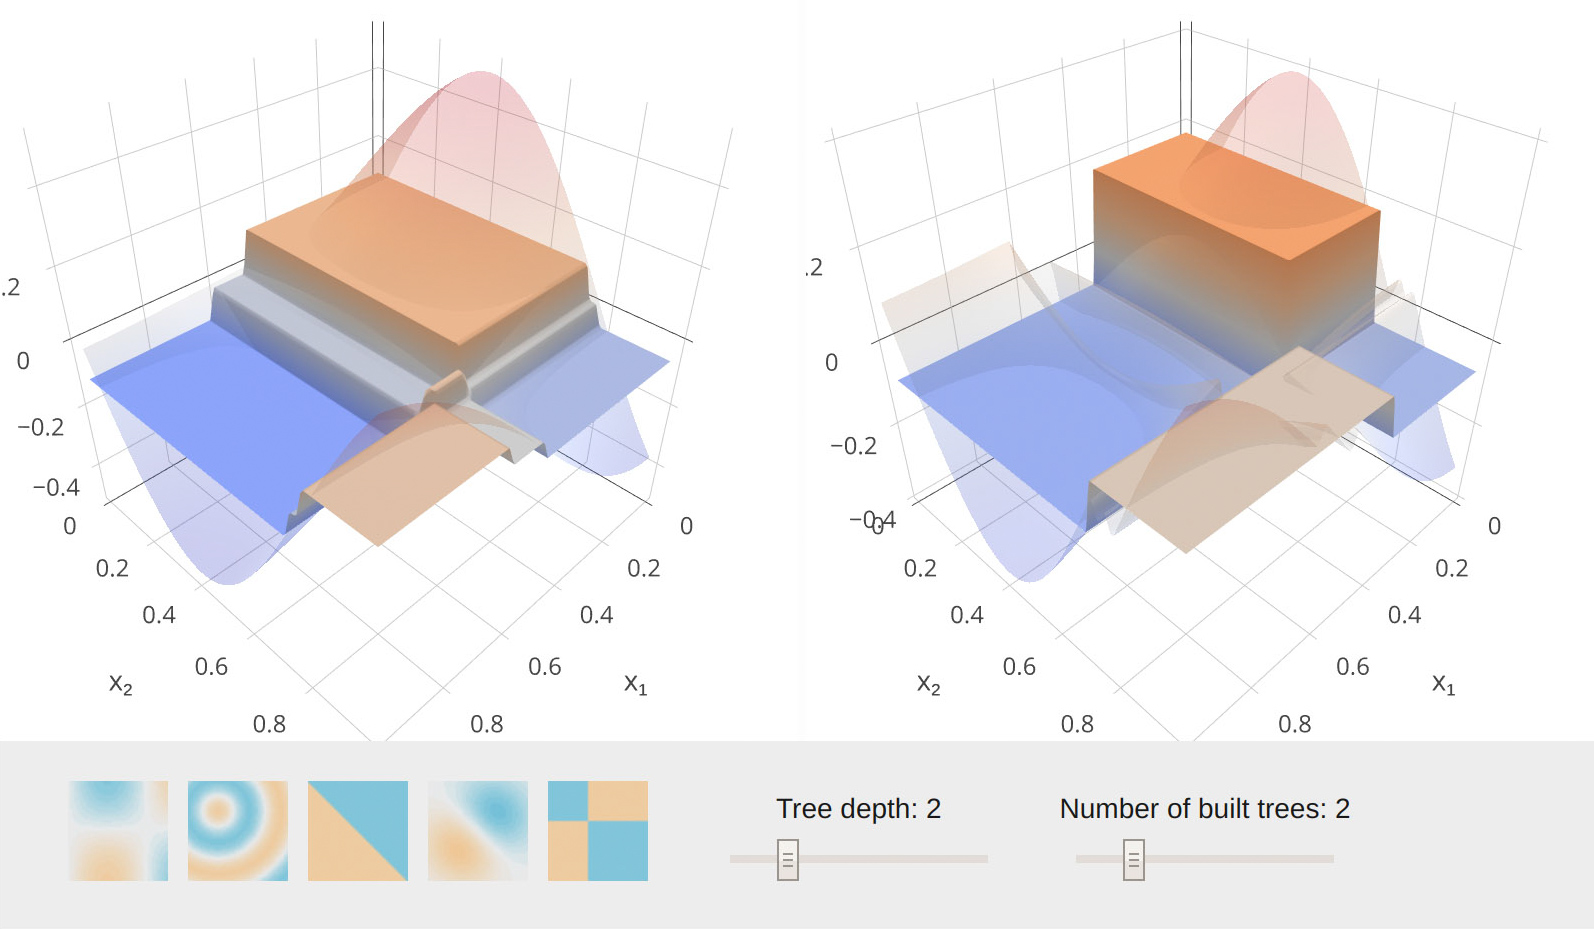
\includegraphics[width=\textwidth]{figure_man/gbm_anim/gbm2.jpg}
% \href{http://arogozhnikov.github.io/2016/06/24/gradient_boosting_explained.html}{\beamergotobutton{Open in browser.}}
% \end{center}
% \addtocounter{framenumber}{-1}
% \end{vbframe}

\begin{vbframe}{Visualization 3}
\begin{center}
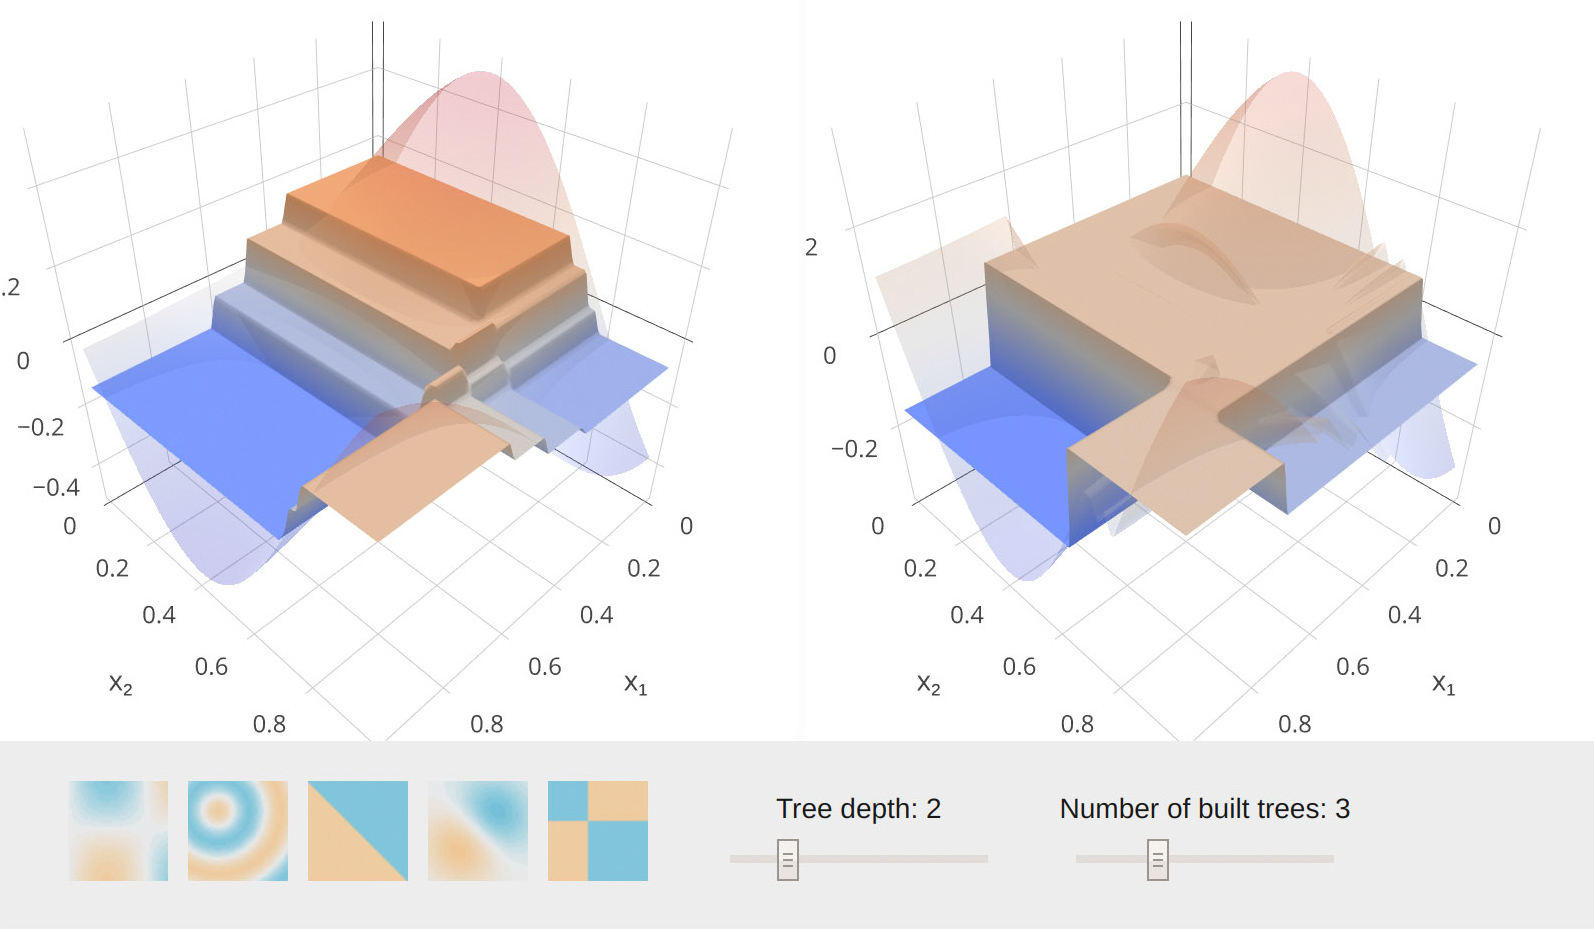
\includegraphics[width=\textwidth]{figure_man/gbm_anim/gbm3.jpg}
\href{http://arogozhnikov.github.io/2016/06/24/gradient_boosting_explained.html}{\beamergotobutton{Open in browser.}}
\end{center}
\addtocounter{framenumber}{-1}
\end{vbframe}

% \begin{vbframe}{Gradient Boosting Visualization}
% \begin{center}
% 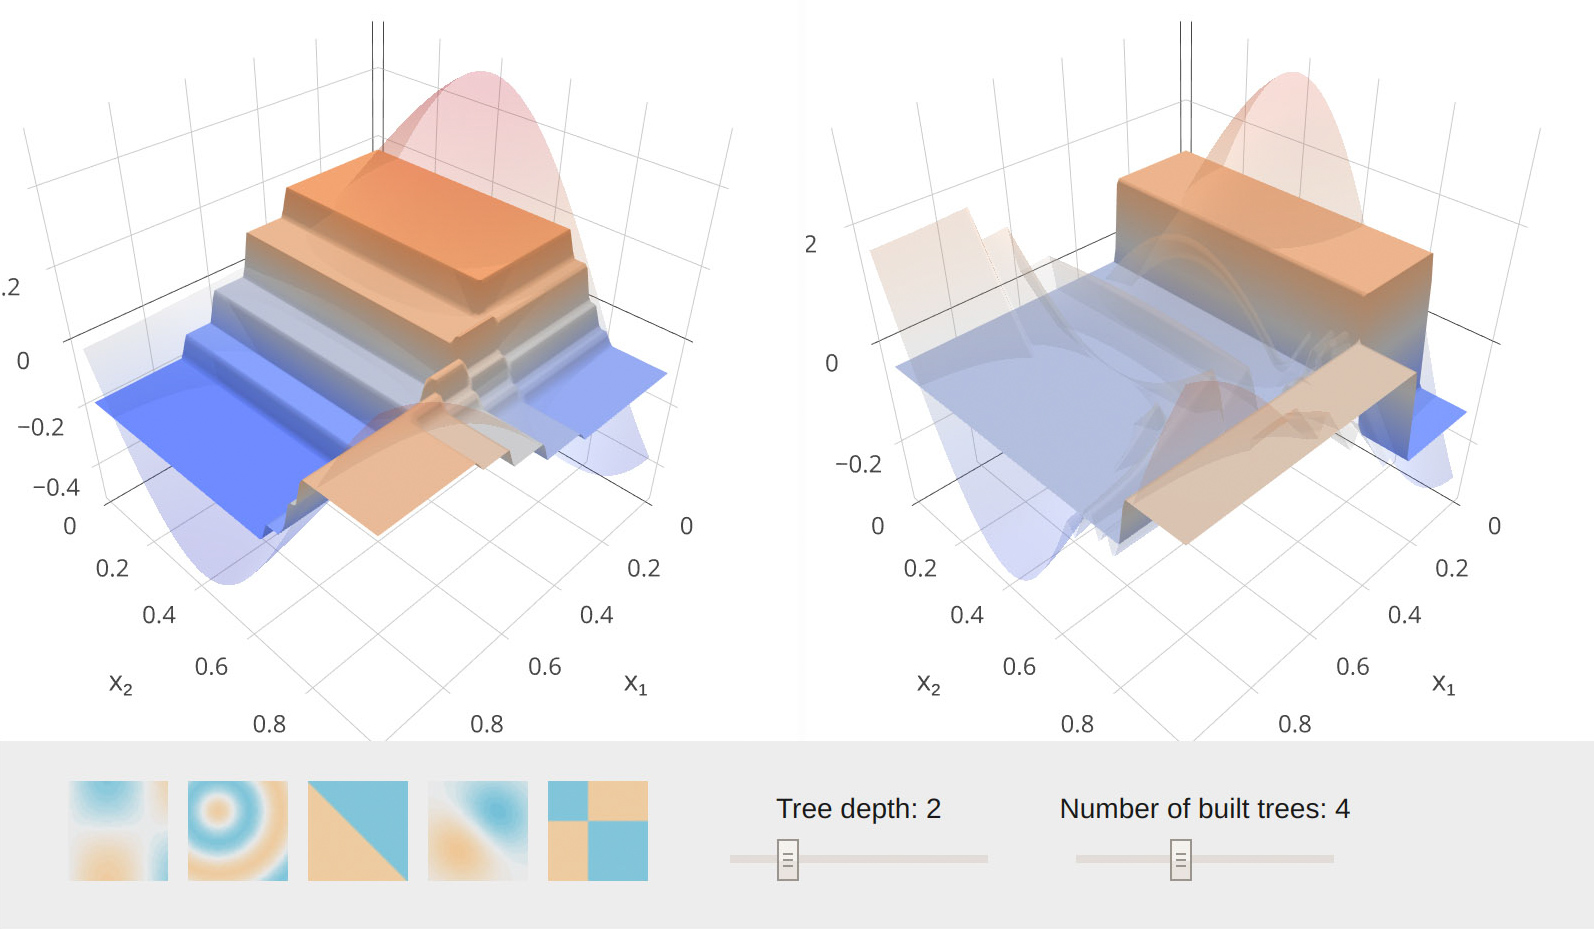
\includegraphics[width=\textwidth]{figure_man/gbm_anim/gbm4.jpg}
% \href{http://arogozhnikov.github.io/2016/06/24/gradient_boosting_explained.html}{\beamergotobutton{Open in browser.}}
% \end{center}
% \addtocounter{framenumber}{-1}
% \end{vbframe}

\begin{vbframe}{Visualization 3}
\begin{center}
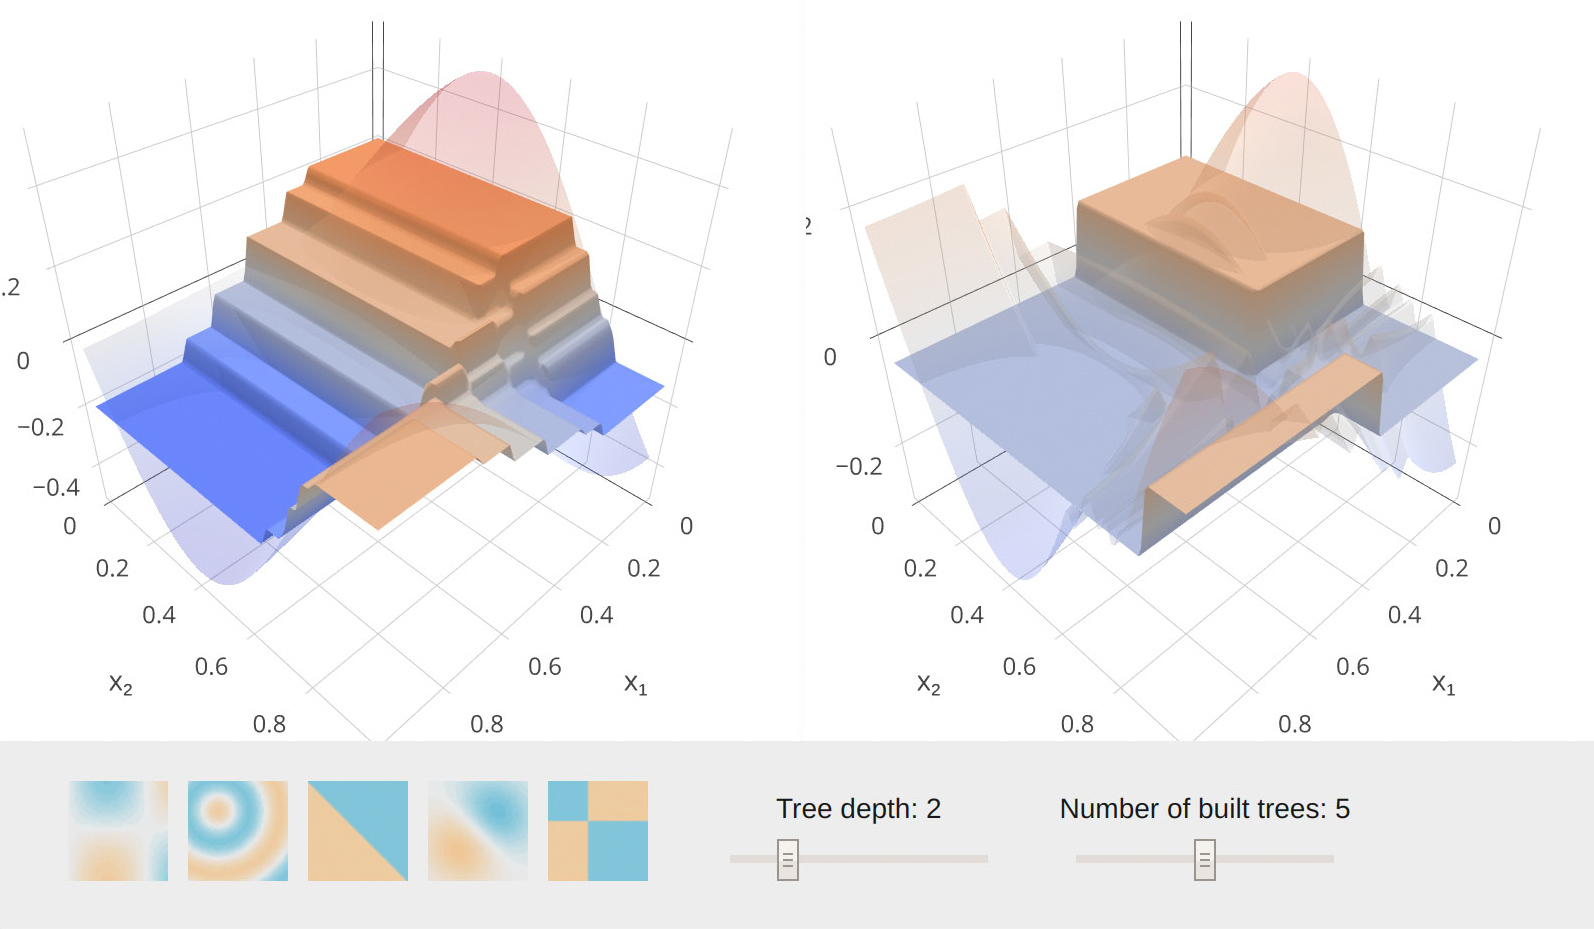
\includegraphics[width=\textwidth]{figure_man/gbm_anim/gbm5.jpg}
\href{http://arogozhnikov.github.io/2016/06/24/gradient_boosting_explained.html}{\beamergotobutton{Open in browser.}}
\end{center}
\addtocounter{framenumber}{-1}
\end{vbframe}

\begin{vbframe}{Visualization 3}
\begin{center}
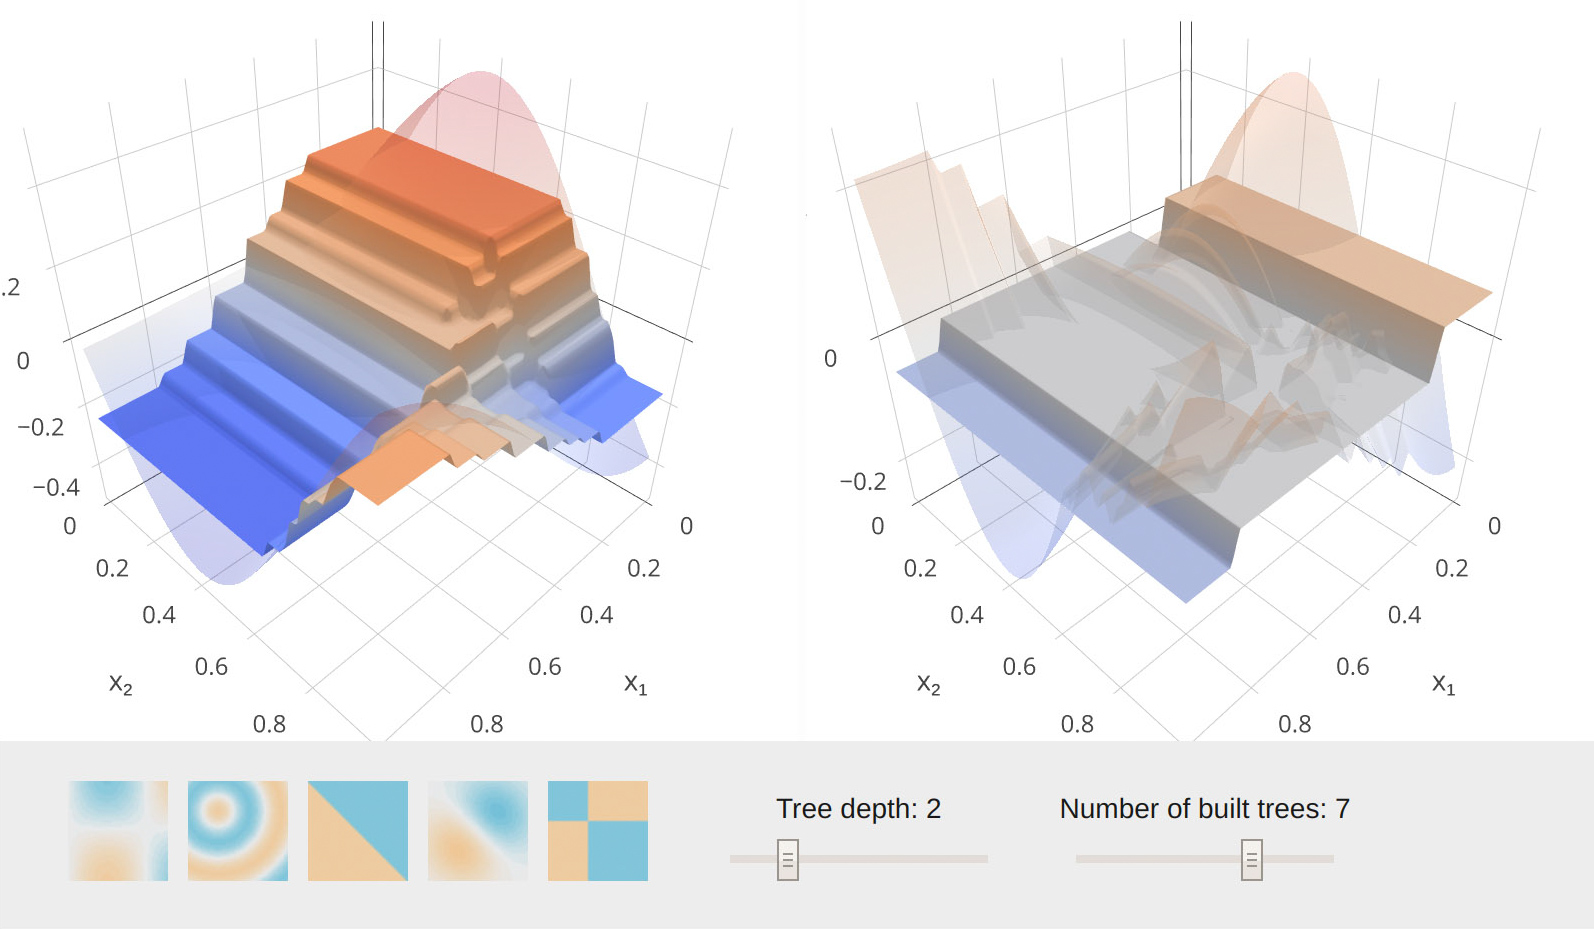
\includegraphics[width=\textwidth]{figure_man/gbm_anim/gbm7.jpg}
\href{http://arogozhnikov.github.io/2016/06/24/gradient_boosting_explained.html}{\beamergotobutton{Open in browser.}}
\end{center}
\addtocounter{framenumber}{-1}
\end{vbframe}

% \begin{vbframe}{Gradient Boosting Visualization}
% \begin{center}
% 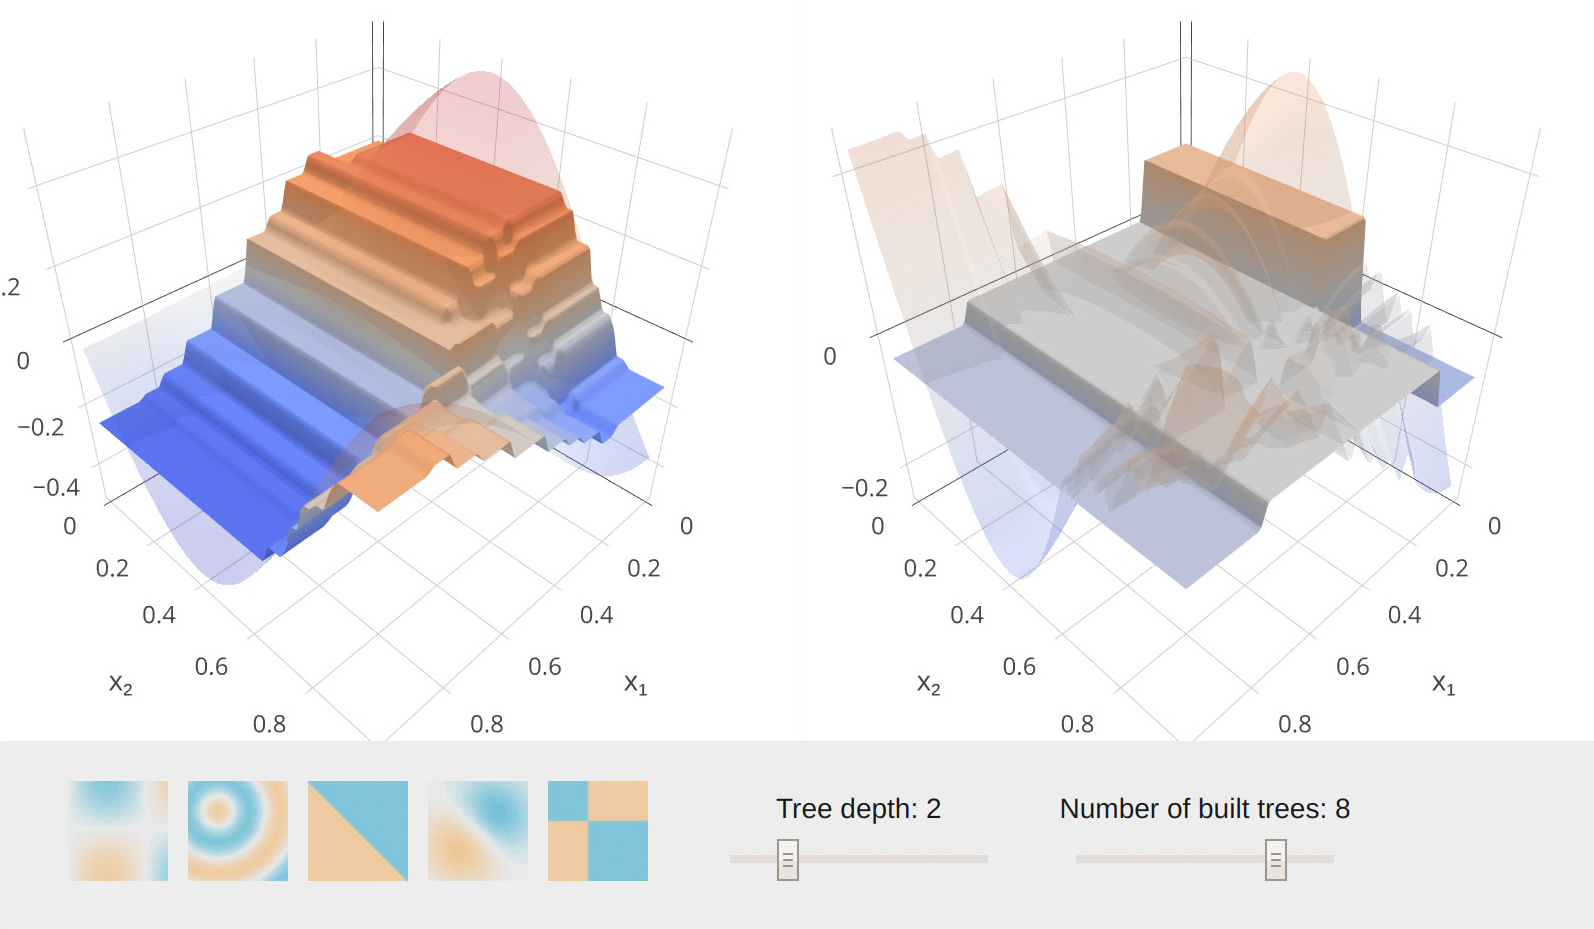
\includegraphics[width=\textwidth]{figure_man/gbm_anim/gbm8.jpg}
% \href{http://arogozhnikov.github.io/2016/06/24/gradient_boosting_explained.html}{\beamergotobutton{Open in browser.}}
% \end{center}
% \addtocounter{framenumber}{-1}
% \end{vbframe}

% \begin{vbframe}{Gradient Boosting Visualization}
% \begin{center}
% 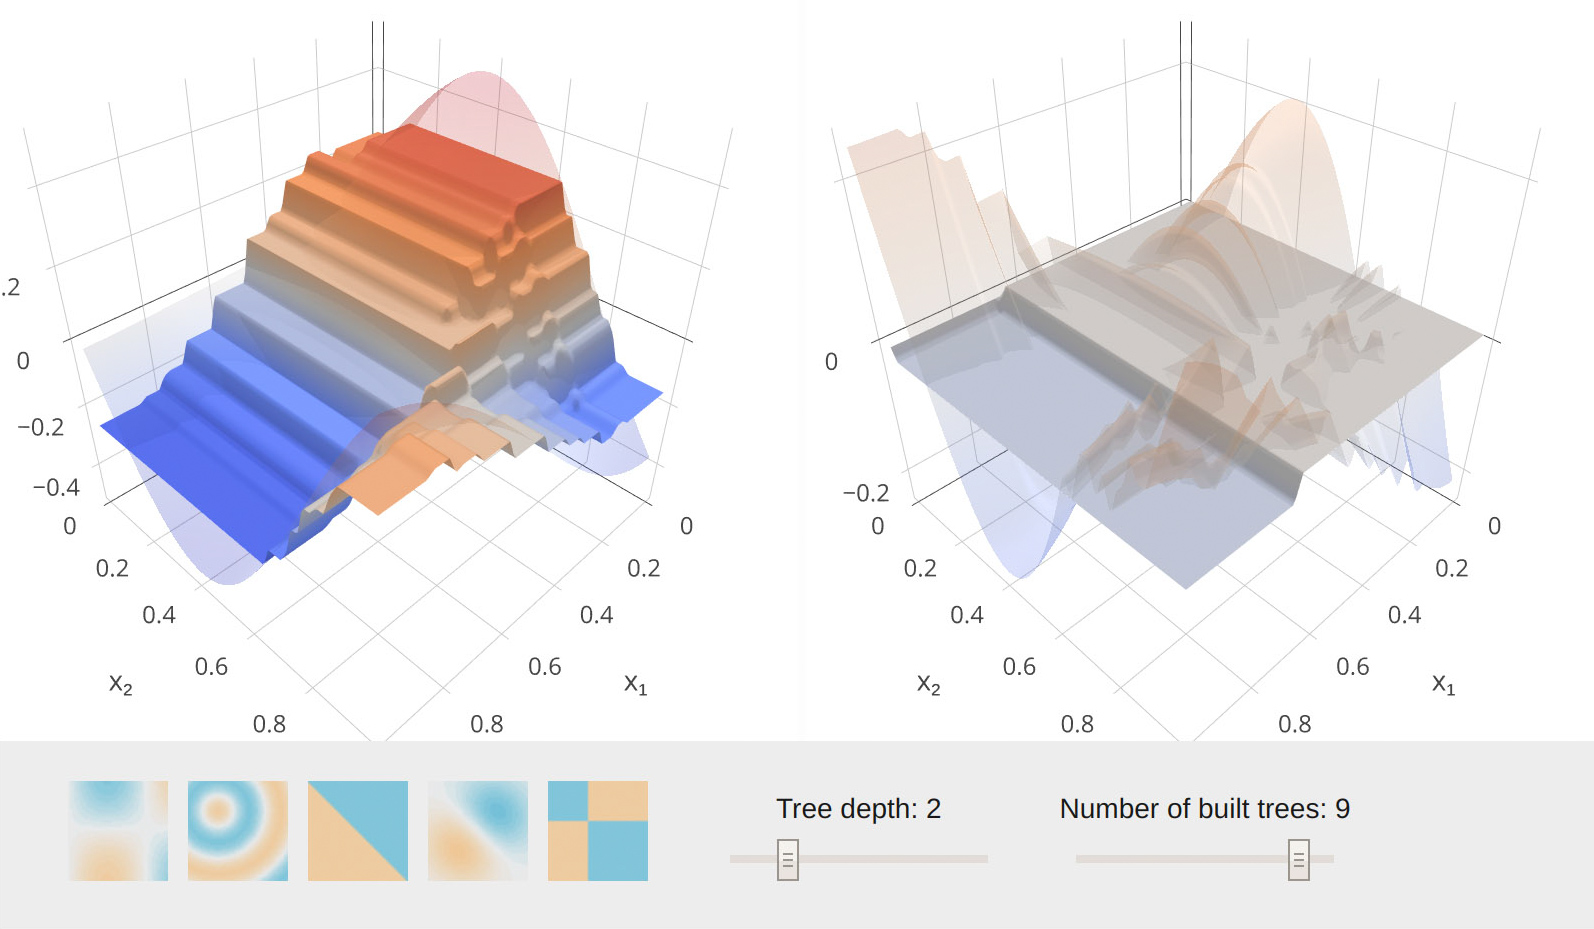
\includegraphics[width=\textwidth]{figure_man/gbm_anim/gbm9.jpg}
% \href{http://arogozhnikov.github.io/2016/06/24/gradient_boosting_explained.html}{\beamergotobutton{Open in browser.}}
% \end{center}
% \addtocounter{framenumber}{-1}
% \end{vbframe}

\begin{vbframe}{Visualization 3}
\begin{center}
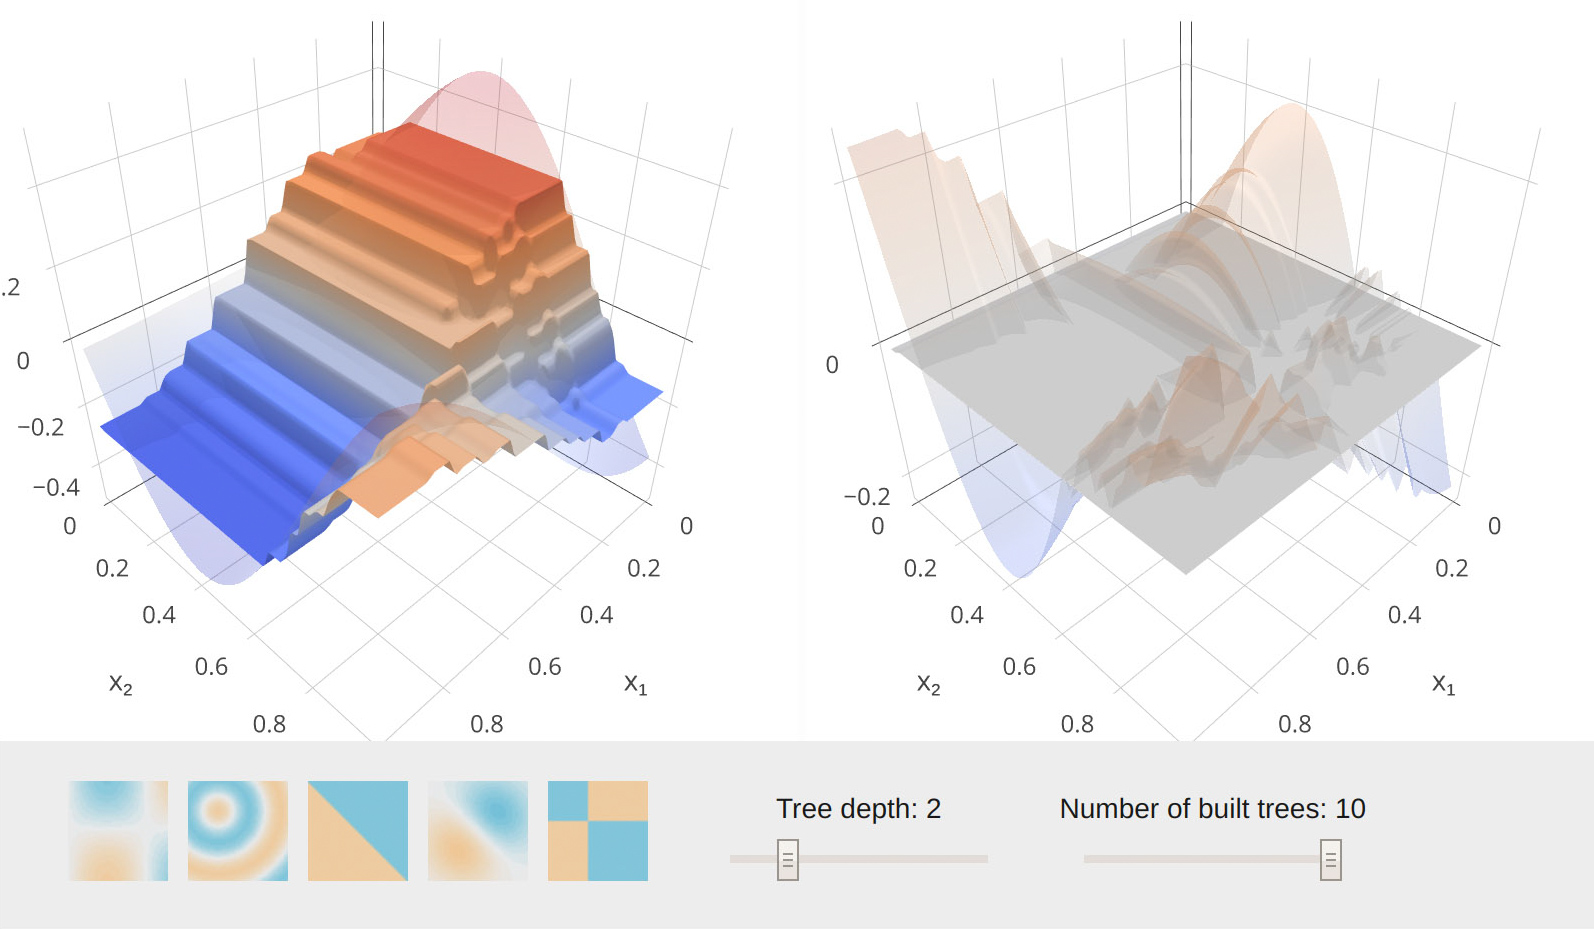
\includegraphics[width=\textwidth]{figure_man/gbm_anim/gbm10.jpg}
\href{http://arogozhnikov.github.io/2016/06/24/gradient_boosting_explained.html}{\beamergotobutton{Open in browser.}}
\end{center}
\addtocounter{framenumber}{-1}
\end{vbframe}


\endlecture
\end{document}
